\documentclass[english,12pt,presentation]{beamer}
\usepackage{graphicx}
\usepackage{beamerthemesplit}
\usepackage{hyperref}
%\setbeameroption{show notes on second screen=right}
\usetheme{Bergen}
%\usetheme{Berkeley}
\useinnertheme{circles}
\useinnertheme{inmargin}
\useoutertheme{infolines}
\usecolortheme{spruce}
\title{Publishing Through Emacs}
\subtitle{Slide Scalable to eBook, Proposal, Report, Journal, Thesis}
\author{Aaron Bello, aaron@hosttor.com, @hosttor}
\date{\today}

\begin{document}
\begin{frame}{Boston Emacs Meetup}
\begin{figure}
\centering
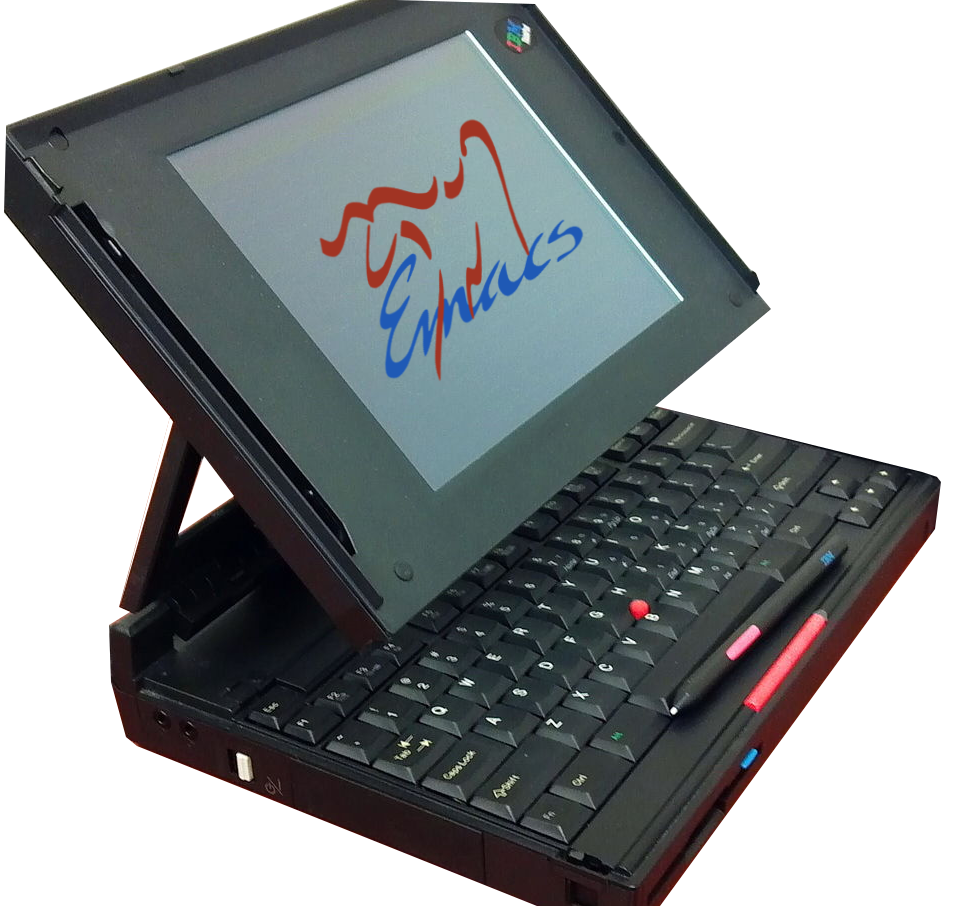
\includegraphics[width=80]{images/emachine.png}
\end{figure}
\titlepage
\end{frame}

\begin{frame}{Proudly Sponsored By}
\begin{figure}
\centering

\includegraphics[width=160]{images/thoughtbot.png}
\item Thoughtbot
\end{figure}
\end{frame}

\begin{frame}{Agenda}
\begin{itemize}
\pause \item Publishing Overview
\pause \item Benefit Of Publishing With eMacs?
\pause \item Profit From Your Hardwork
\pause \item Demostration Time
\pause \item Questions
\end{itemize}
\end{frame}

\begin{frame}{Publishing Overview}
\begin{itemize}
\pause \item Produce a very fast, free, scalable slide with ease.
\pause \item Create a stunning cover image for ebook
\pause \item Create a METADATA (Title, Author Name, Category, Description, Language, Tags, ISBN and Pub Date)
\pause \item Compile to Slide, eBook, Proposal, Journal, Report, Thesis etc
\pause \item Obtain ISBN and Copyright
\pause \item Distribute to public libraries and global marketplace
\pause \item Marketing and Advertising
\end{itemize}
\end{frame}

\begin{frame}{Benefit Of Publishing With eMacs?}
\begin{itemize}
\pause \item Total control of production
\pause \item Short time of production
\pause \item Low or Zero cost of production
\pause \item Supereasy to produce
\pause \item Reproduceable
\end{itemize}
\end{frame}

\begin{frame}{Profit From Your Hardwork}
Millions of buyers are on the global marketplace such as;
\begin{itemize}
\pause \item Global Distributor: \pause Barnes and Nobles, \pause Baker and Taylor, \pause Overdrive, \pause Amazon, \pause Google, \pause Scribd, \pause Apple, \pause ingram, \pause iBook, \pause Kobo, \pause Sony etc
\pause \item Online Service for Nongeek: Clickbank, \pause Payhip, \pause Lulu, \pause e-junkie, \pause Smashwords, \pause Booktango, \pause Bookbaby, \pause Myebook, \pause Blurb, \pause Txtr, \pause flipkart, \pause Page \pause foundry, \pause Blio, \pause ebookmall, \pause PayLoadz, \pause click2sell, \pause instabuck, \pause payspree etc
\end{itemize}
\end{frame}

\begin{frame}{Demostration Time}
\begin{figure}
\centering
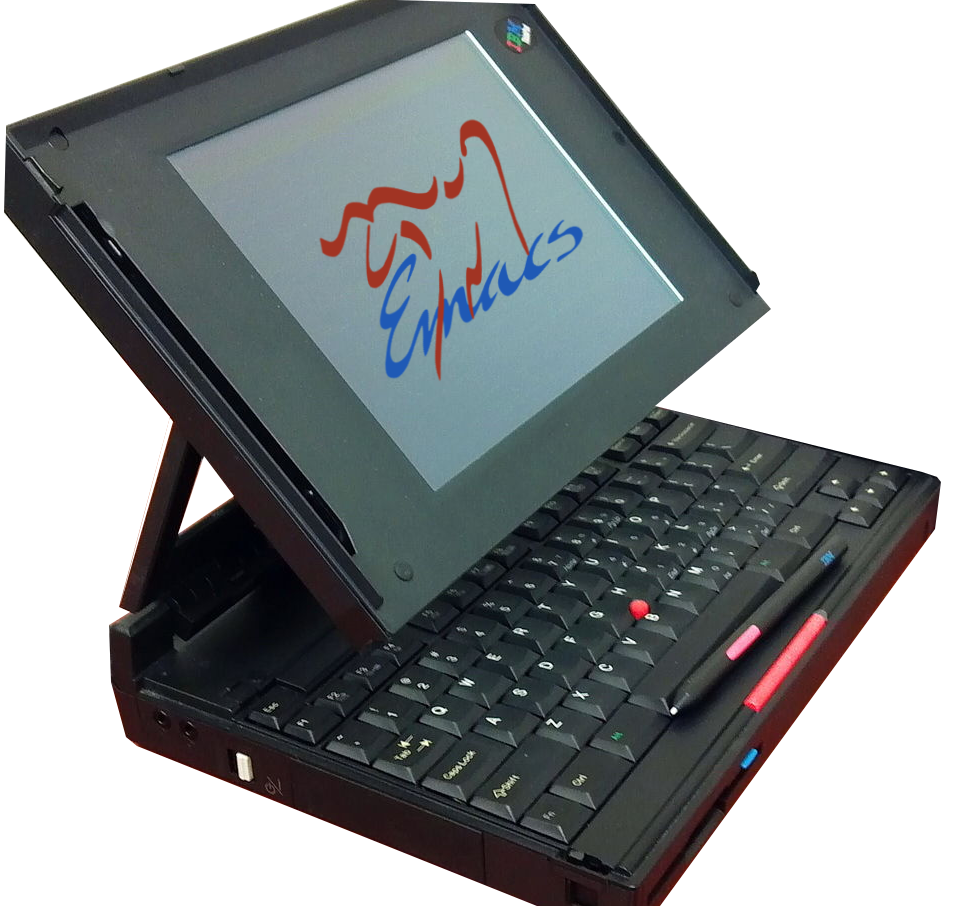
\includegraphics[width=220]{images/emachine.png}
\end{figure}
\titlepage
\end{frame}

\begin{frame}{Using LaTex and Beamer for production}
LaTex is a powerful program used in \pause Computing, \pause Engineering, \pause Mathematics and Science, \pause Theorems, \pause Chemical Graphics, \pause Source Code Listings, \pause Letters, \pause Proposal, \pause Advanced Mathematics etc.
\begin{itemize}
\pause \item documentclass
\pause \item usepackage
\pause \item usetheme \pause useinnertheme
\pause \item title, \pause subtitle, \pause author \pause and date
\pause \item begin document, \pause end document
\pause \item begin frame, \pause end frame, \pause pause item
\pause \item begin figure, \pause includegraphics \pause end figure
\end{itemize}
\end{frame}

\begin{frame}{Thank you all for coming}
\begin{figure}
\centering

\includegraphics[width=220]{images/thanks.png}
\end{figure}
\item Thank you! Thank you!! Thank you!!!
\end{frame}

\begin{frame}{Stay Connected!!!}
\begin{itemize}
\item \url{https://www.hosttor.com/}
\item \url{https://linkedin.com/company/hosttor/}
\item \url{https://www.twitter.com/hosttor/}
\item \url{https://www.facebook.com/hosttor/}
\item \url{https://hosttor.tumblr.com/}
\item \url{https://www.pinterest.com/hosttor/}
\end{itemize}
\end{frame}

\begin{frame}{QUESTIONS?}
\begin{figure}
\centering

\includegraphics[width=220]{images/q.png}
\end{figure}
\end{frame}
\end{document}